\documentclass{standalone}
\usepackage{tikz}

\begin{document}
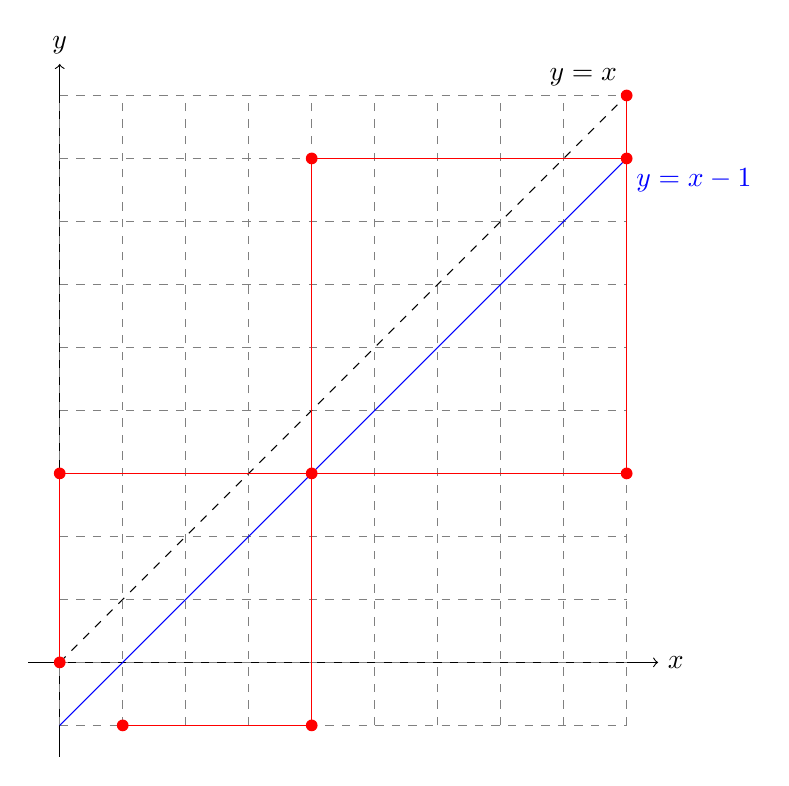
\begin{tikzpicture}[scale=0.8]
    % Axes
    \draw[->] (-0.5,0) -- (9.5,0) node[right] {$x$};
    \draw[->] (0,-1.5) -- (0,9.5) node[above] {$y$};

    % Grid lines
    \foreach \x in {0,...,9}
    \draw[dashed, gray] (\x cm,-1) -- (\x cm,9);
    \foreach \y in {-1,...,9}
    \draw[dashed, gray] (0,\y cm) -- (9,\y cm);


    % Line y=x
    \draw[dashed, black] (0,0) -- (9,9) node[above left] {$y=x$};
    % Line y=x-1
    \draw[blue] (0,-1) -- (9,8) node[below right] {$y=x-1$};



    % Red arc from (0,0) to (2,2)
    \draw[red] (0,0) to (0,3);
    \draw[red] (1,-1) to (4,-1);
    \draw[red] (0,3) to (4,3);
    \draw[red] (4,-1) to (4,3);
    \draw[red] (4,3) to (4,8);
    \draw[red] (4,3) to (9,3);
    \draw[red] (9,3) to (9,8);
    \draw[red] (4,8) to (9,8);
    \draw[red] (9,8) to (9,9);
    % \draw[red] (4,4) to[out=90,in=180] (9,9);


    % Red point at (2,2)
    \node[circle, fill=red, inner sep=1.5pt] at (0,0) {};
    \node[circle, fill=red, inner sep=1.5pt] at (1,-1) {};
    \node[circle, fill=red, inner sep=1.5pt] at (0,3) {};
    \node[circle, fill=red, inner sep=1.5pt] at (4,3) {};
    \node[circle, fill=red, inner sep=1.5pt] at (4,-1) {};
    \node[circle, fill=red, inner sep=1.5pt] at (4,8) {};
    \node[circle, fill=red, inner sep=1.5pt] at (9,3) {};
    \node[circle, fill=red, inner sep=1.5pt] at (9,8) {};
    \node[circle, fill=red, inner sep=1.5pt] at (9,9) {};

\end{tikzpicture}
\end{document}
